
\section{Parallel Scaling of the EMG model in High Performance Computing}
% in opendihu 2021 paper

After the parallel scaling of the multi-scale model in moderately parallel scenarios up to 27 processes has been investigated in the previous sections, we now study the parallel scalability in High Performance Computing scenarios with larger degrees of parallelism.
We conduct these studies on the supercomputer Hawk at the High Performance Computing Center Stuttgart (HLRS). 

In the following, \cref{sec:weak_scaling_hawk} presents a weak scaling study, which scales the problem size up to a realistic number of \num{270000} muscle fibers.
Then, \cref{sec:mpi_rank_placement} shows measurements of the scaling behavior for the 1D model solver and gives details on MPI rank placement policies.

\subsection{Weak Scaling of the Fiber Based Electrophysiology Model}\label{sec:weak_scaling_hawk}

We simulate the fiber based electrophysiology model with EMG values on the muscle surface and the subcellular model of Hodgkin and Huxley \cite{Hodgkin1952}.
Corresponding simulation results of this scenario, also for the highly parallel runs, are presented in \cref{sec:effects_of_the_mesh_width_emg}.

In this weak scaling study, the number of fibers and number of processes is varied while their relation is kept approximately constant. The scenarios are chosen such that there are approximately 10 fibers per process, while maintaining a cube-liked partitioning scheme in the 3D domain. The 0D subcellular and the 1D electric conduction problems on the fibers are solved with the \code{FastMonodomainSolver} class and the \code{`vc`} optimization type, which is the fastest available option in OpenDiHu. The Strang operator splitting scheme with Heun's method and the implicit Euler scheme are used. The 3D problem is solved using the conjugate gradient solver of PETSc and a relative tolerance on the residual norm of \num{1e-5}. 

The used timestep widths are $\dt_\text{0D}=\SI{1e-3}{\milli\second}$, $\dt_\text{1D}=\dt_\text{splitting}=\SI{2e-3}{\milli\second}$ and $\dt_\text{3D}=\SI{1}{\milli\second}$. Because only the scaling behaviour is of interest in this study, the simulation end time is set to $t_\text{end}=\SI{2}{\milli\second}$.

% Hawk weak scaling
\begin{figure}[H]
  \centering%
  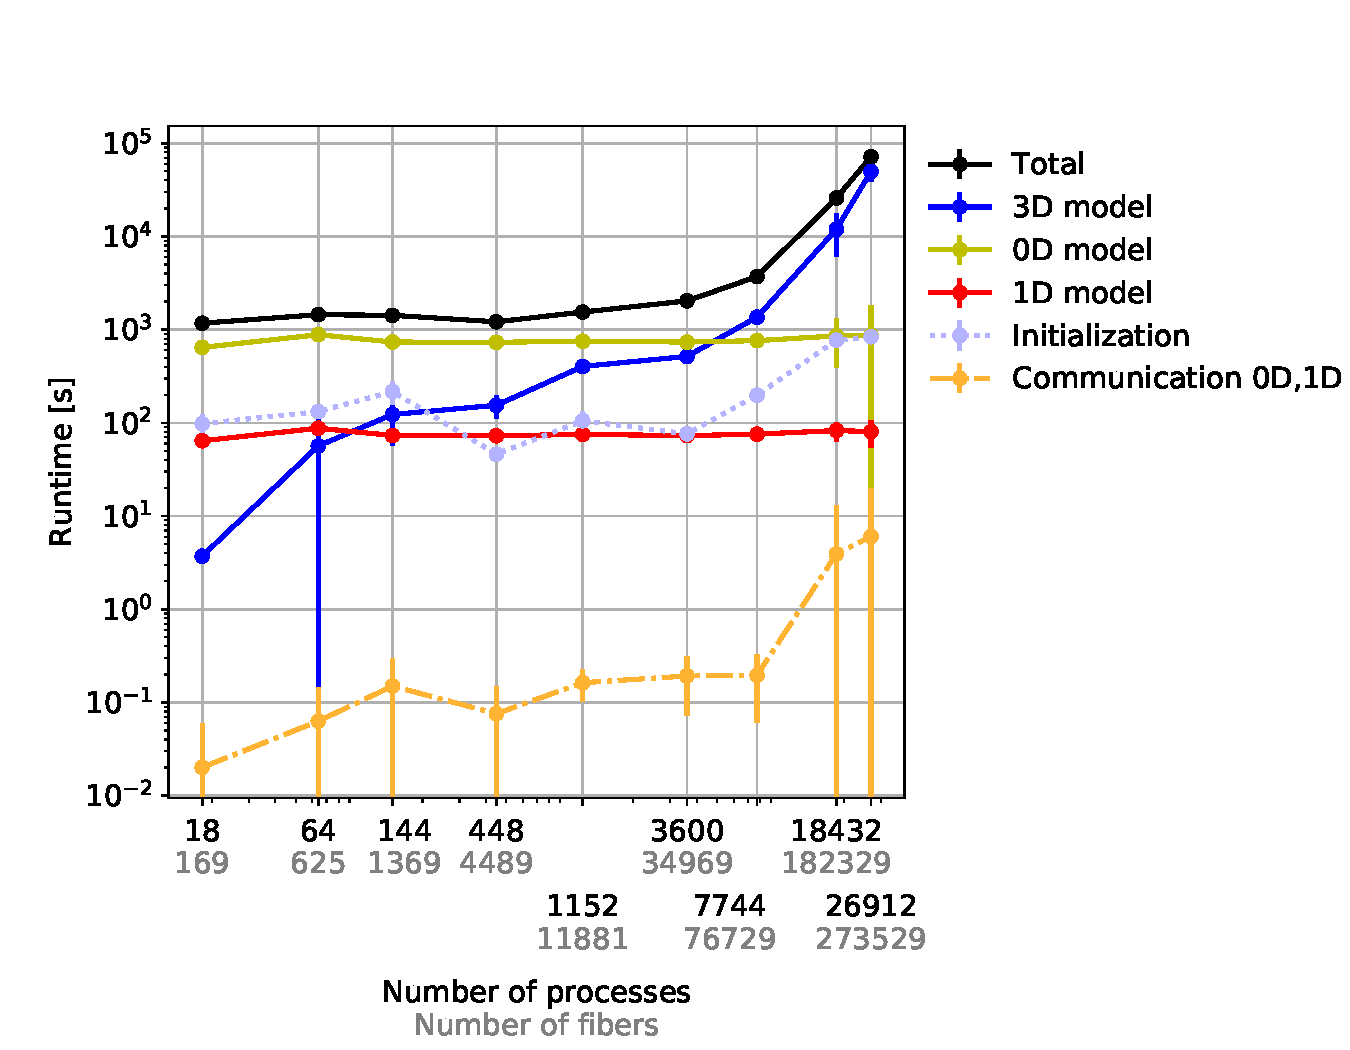
\includegraphics[width=\textwidth]{images/results/studies/hawk_weak_scaling.pdf}%
  \caption{Weak scaling of the fiber based electrophysiology model on the supercomputer Hawk simulating up to more than \num{270000} muscle fibers.}%
  \label{fig:hawk_weak_scaling}%
\end{figure}

\Cref{fig:hawk_weak_scaling} presents the resulting runtimes for the different parts of the simulation program: the solvers of the 0D, 1D and 3D models, the runtime for initialization and the runtime for the communication in the \code{FastMonodomainSolver}, as explained in \cref{sec:improved_parallel_solver_for_fiber_based}.
To relate the initialization runtime to the runtime of the solvers in a realistic scenario with longer simulation times, all runtimes except for the initialization are scaled to a simulation end time of $\SI{1}{\second}$.

The results show perfect weak scaling properties of the 0D and 1D solvers, given by the yellow and red lines. Both is expected due to the construction and the parallel partitioning. The 0D problems are \say{embarassingly parallel} and are solved independent of each other. In the 1D problem solver, the values are  transferred to a dedicated process, where the serial Thomas algorithm is employed. Thus, the solution of all 1D problems is also performed independent of each other, except for the communication cost.
The plot shows a very small runtime for this communication, which is given by the orange dashed line, even for higher parallelism.

The time for initialization involves parsing the Python script, which for the last data point requires \SI{35.1}{\s}, parallel file access and read operations of the mesh file, assembly of the 3D stiffness matrix and solution of the potential flow problem to obtain the fiber directions in the 3D mesh, which contains approximately \num{1e8} dofs for the last data point, code generation, compilation, linking and loading of the shared library for the subcellular problem, and initialization of all internal data structures.

Loading the mesh input file from the file system is the part of the initialization that requires the most runtime.
The dotted light blue line in \cref{fig:hawk_weak_scaling} shows that the initialization time increases to a maximum value of \SI{839}{\s} for the largest problem size.

The runtime of the 3D model is shown by the blue line in \cref{fig:hawk_weak_scaling}. This part of the model is responsible for the highest portion of the total runtime starting from the scenario with \num{7744} fibers and \num{76729} processes. This increase is two-fold: first, the communication cost increases for a larger number of processes. Second, the number of iterations in the conjugate gradient solver increases for a larger number of unknowns.

\begin{table}
  \centering%
  \begin{tabular}{|r|r|r|r|r|r|r|r|r|}
    \hline
    \# processes  & 18 & 64  & 144 & 448  & 1152 & 3600 & 7744 & \num{26912}\\\hline
    \# iterations & 72 & 115 & 176 & 339  & 561  & 1056 & 1636 & 2807\\
    \hline
  \end{tabular}
  \caption{Number of iterations of the conjugate gradient solver for the weak scaling study presented in \cref{fig:hawk_weak_scaling}.}%
  \label{tab:cg_solver_iterations}%
\end{table}

In this weak scaling study, the number of conjugate gradient solver iterations increases from 72 for the first data point to \num{2807} for the last data point, as listed in \cref{tab:cg_solver_iterations}. The 3D problem of the last data point has \num{1e9} dofs. The exact numbers of dofs are also listed in \cref{tab:emg_study_parameters} in \cref{sec:effects_of_the_mesh_width_emg}.
Currently, the solution of the 3D problem uses no preconditioner. In future work, a multigrid solver could be employed for preconditioning, which could improve the weak scaling for large problem sizes.

In summary, the solution of the multi-scale model for fiber based electrophysiolgy without fat layer exhibits a very good weak scalability for up to \num{35e3} fibers. For larger problem sizes, the solution of the 3D problem dominates and the weak scaling behavior deteriorates. However, the solution times are still feasible, as such large problems have been successfully solved in \cref{sec:effects_of_the_mesh_width_emg} of this work.


%         n_it
% nRanks      
% 18        72
% 64       115
% 144      176
% 448      339
% 1152     561
% 3600    1056
% 7744    1636
% 26912   2807

% partitioning  2* 2* 1=    4    7^2=    49 fibers, fibers/rank: 12.250000, need    1 nodes
% partitioning  3* 3* 2=   18   13^2=   169 fibers, fibers/rank: 9.388889, need    1 nodes
% partitioning  4* 4* 4=   64   25^2=   625 fibers, fibers/rank: 9.765625, need    1 nodes
% partitioning  6* 6* 4=  144   37^2=  1369 fibers, fibers/rank: 9.506944, need    3 nodes
% partitioning  7* 8* 8=  448   67^2=  4489 fibers, fibers/rank: 10.020089, need    7 nodes
% partitioning 12*12* 8= 1152  109^2= 11881 fibers, fibers/rank: 10.313368, need   18 nodes
% partitioning 15*15*16= 3600  187^2= 34969 fibers, fibers/rank: 9.713611, need   57 nodes
% partitioning 22*22*16= 7744  277^2= 76729 fibers, fibers/rank: 9.908187, need  121 nodes
% partitioning 24*24*32=18432  427^2=182329 fibers, fibers/rank: 9.891981, need  288 nodes
% partitioning 29*29*32=26912  523^2=273529 fibers, fibers/rank: 10.163830, need  421 nodes
% partitioning 40*40*32=51200  523^2=273529 fibers, fibers/rank: 5.342363, need  800 nodes
%                                           subdomains        user  total comp.        0D        1D   bidomain  duration_init  write       mem  n_it      n
% scenarioName                    nRanks                                                                                                                   
% hawk_weak_scaling_endtime_1.0_1 18         [3, 3, 2]  100.216111     2.346004  1.289333  0.128295   0.007430      97.870107    0.0  0.203 GB    72     18
%                                 64         [4, 4, 4]  134.937500     2.893596  1.765827  0.175330   0.113093     132.043904    0.0  0.315 GB   115     64
%                                 144        [6, 6, 4]  219.409583     2.850457  1.473133  0.146266   0.245577     216.559126    0.0  0.341 GB   176    144
%                                 448        [7, 8, 8]   48.533839     2.428730  1.463591  0.145278   0.308863      46.105109    0.0  0.584 GB   339    448
%                                 1152     [12, 12, 8]  295.241211     3.548350  1.489827  0.148680   1.321491     291.692861    0.0  0.385 GB   561   2304
%                                 3600    [15, 15, 16]   80.168103     4.069231  1.471832  0.146008   1.033123      76.098872    0.0  0.955 GB  1056   3600
%                                 7744    [22, 22, 16]  205.599181     7.422947  1.524253  0.151227   2.725283     198.176234    0.0  1.001 GB  1636   7744
%                                 18432   [24, 24, 32]  823.224210    51.681839  1.714082  0.165388  23.903565     771.542371    0.0  1.921 GB     0  18432
%                                 26912   [29, 29, 32]  982.392875   143.146126  1.739032  0.161190  99.627309     839.246749    0.0  2.066 GB  2807  26912

%-----
\subsection{Weak Scaling of the 1D Solver and MPI Rank Placement}\label{sec:mpi_rank_placement}


% performance/opendihu/08_0D1D_better_implementation
Next, we compare the different approaches to solve the 1D electric conduction part of the monodomain equation on the fibers.
\Cref{fig:hazel_hen_rank_placement} shows a similar weak scaling study to the one in the last section with slightly different process counts. The study was carried out on the supercomputer Hazel Hen, Cray XC30 which was installed until 2020 at the High Performance Computing Center Stuttgart. The same problem as in the last section is solved, and, again, the relation between fibers and processes is 10:1. The partitionings were chosen in accordance with the compute nodes of Hazel Hen, which had 24 cores. The detailed problem sizes and partitionings can be found in \cite{Maier2019}.

\Cref{fig:hazel_hen_rank_placement} shows the runtimes of the same 0D and 1D solvers as in the last section by the solid yellow line for the 0D problem, the solid red line below for the 1D problem and the solid orange line for the communication. The perfect weak scaling for these parts is in line with the previous observations.

\begin{figure}
  \centering%
  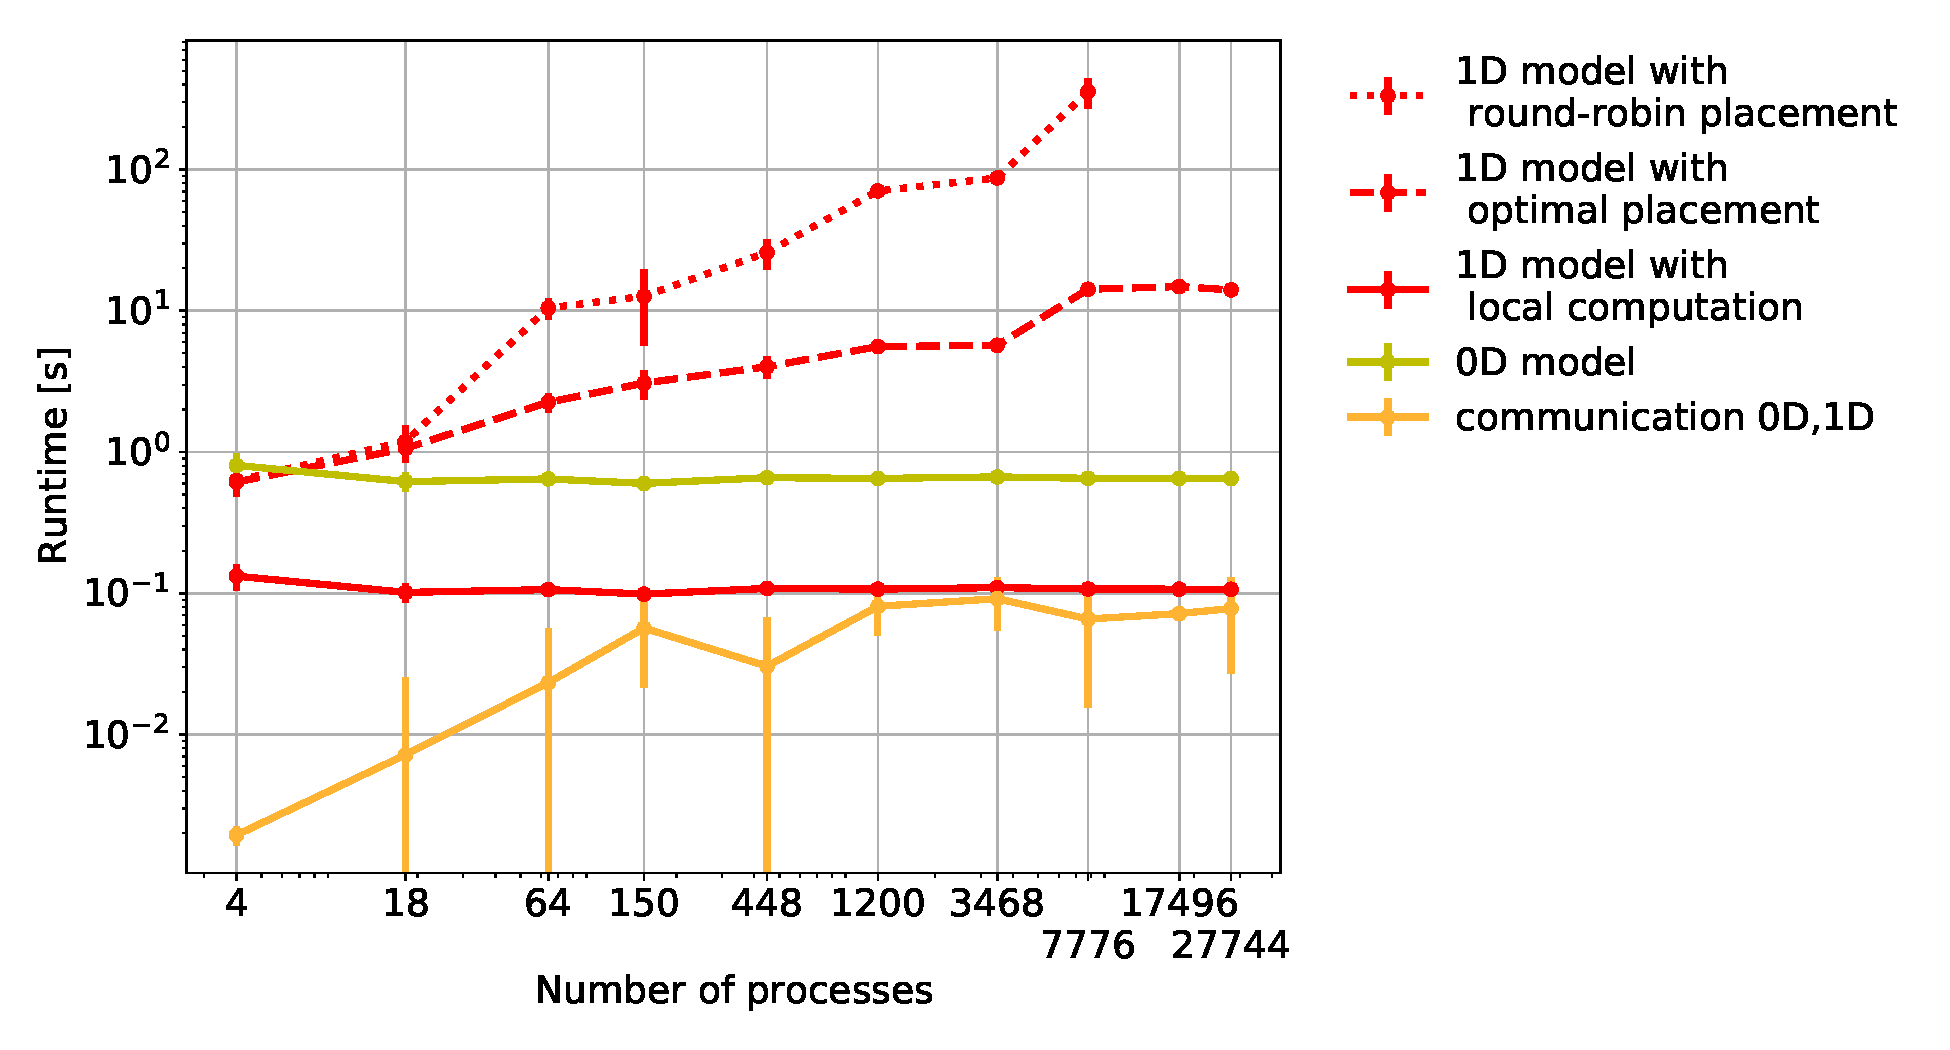
\includegraphics[width=\textwidth]{images/results/studies/Comparisonof0D-1Dcomputationschemes.pdf}%
  \caption{Rank placement strategy}% 
   \label{fig:hazel_hen_rank_placement}%
\end{figure}

In addition, we compare the weak scaling of the 1D solution if a parallel conjugate gradient solver of PETSc is used for the problem on every fiber, instead of the serial Thomas algorithm. This setup corresponds to the \code{vc-aovs} scenario presented in \cref{sec:evaluation_of_code_gen}. As already noted earlier, the performance of this approach is worse. The dashed and dotted lines in \cref{fig:hazel_hen_rank_placement} present the runtime of this approach for two different MPI rank placement strategies, but for the identical program. It can be seen that the runtime increases with higher numbers of processes in both curves. This effect is the result of the 1D fiber problems being distributed to more processes, as the total number of processes increases. 

For example, in the scenarios with 1200 and 3468 processes, all fibers are distributed to 12 different processes. For the last three data points of the dashed curve, all fibers are distributed to 24 processes. As a result, the runtime to solve the 1D problems in the measurements with 1200 and 3468 processes is approximately equal, but lower than the runtime for the last three data points, where twice the amount of processors take part in the solution of a single 1D problem.

The difference between the dotted and dashed red curves is a different strategy to place the processes on the compute nodes. The dashed curve with the lower runtime corresponds to a placement of all the processes that share fibers on the same compute node. As the subdomain indices in the $n_x \times n_y \times n_z$ partitioning increase fastest in $x$-direction, then in $y$-direction and then in $z$-direction and the fibers are aligned with the $z$ direction, the set of processes on a compute node contains MPI ranks that are offset with a constant stride of $n_x\,n_y$. This has to be ensured by explicit rank pinning to the compute nodes.

If no such measures are taken, the default placement of MPI ranks to compute nodes occurs consecutively by filling the compute nodes in order. This corresponds to a round-robin placement of the MPI ranks that compute the same fiber, which is the worst possible way of distributing MPI ranks to compute nodes. All processes that compute a fiber are all located on different nodes and have to communicate over compute node boundaries.
\Cref{fig:hazel_hen_rank_placement} shows the resulting runtimes by the upper, dotted red curve. The difference in runtime increases to one order of magnitude with higher number of cores.

Thus, it is important to properly handle MPI rank placement on compute clusters with multiple compute nodes. In consequence, we also configured rank placement on the supercomputer Hawk accordingly in all our studies on this system.

\section{Performance Studies of the Solid Mechanics Solver}

TODO

% numeric investigations
\section{Studies of Numeric Properties}

Next, we perform numeric studies to evaluate used mesh resolutions and solvers. 
\Cref{sec:action_potential_velocity} addresses the mesh width of the 1D problem. Then, \cref{sec:multidomain_solvers} evaluates different numerical solver choices for the multidomain model.

\section{Effect of the Mesh Width on the Action Potential Propagation Velocity}\label{sec:action_potential_velocity}

The numeric parameters of a simulation scenario, such as mesh widths and timestep widths should be chosen such that the resulting numerical errors are balanced between all model components. In the simulation of activated muscle fibers, the propagation velocity of the action potentials is an important quantity, which also influences the macroscopic outcome of EMG recordings. Thus, we investigate the effect of numerical parameters on the propagation velocity.

%performance/opendihu/02_propagation_velocity
\begin{figure}%
  \centering%
  \begin{subfigure}[t]{0.45\textwidth}%
    \centering%
    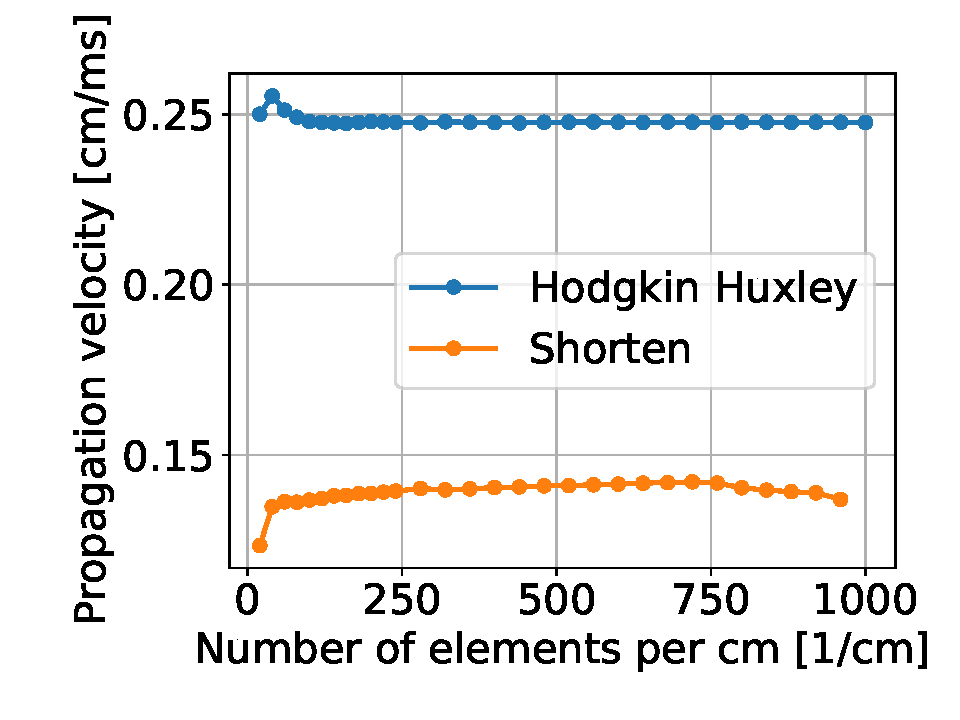
\includegraphics[width=\textwidth]{images/results/studies/propagation_velocity.pdf}%
    \caption{Propagation velocities over spatial resolution of the 1D mesh.}%
    \label{fig:propagation_velocity_comparison}%
  \end{subfigure}
  \,
  \begin{subfigure}[t]{0.45\textwidth}%
    \centering%
    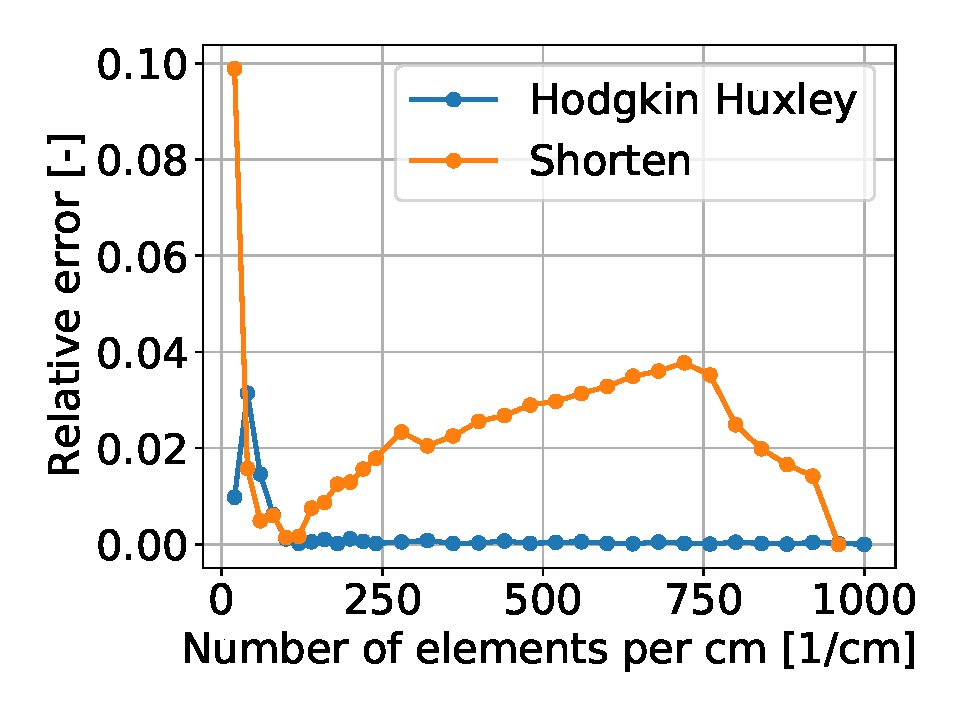
\includegraphics[width=\textwidth]{images/results/studies/propagation_velocity_rel_error.pdf}%
    \caption{Relative error of the propagation velocities over spatial resolution of the 1D mesh.}%
    \label{fig:propagation_velocity_rel_error}%
  \end{subfigure}   
  \caption{Propagation velocities of action potentials for the subcellular models of Shorten and Hodgkin-Huxley. This study is used to determine the 1D mesh width.}%
  \label{fig:propagation_velocity}%
\end{figure}%



\Cref{fig:propagation_velocity} 

%performance/opendihu/03_dx_dt_dependence
\begin{figure}
  \centering%
  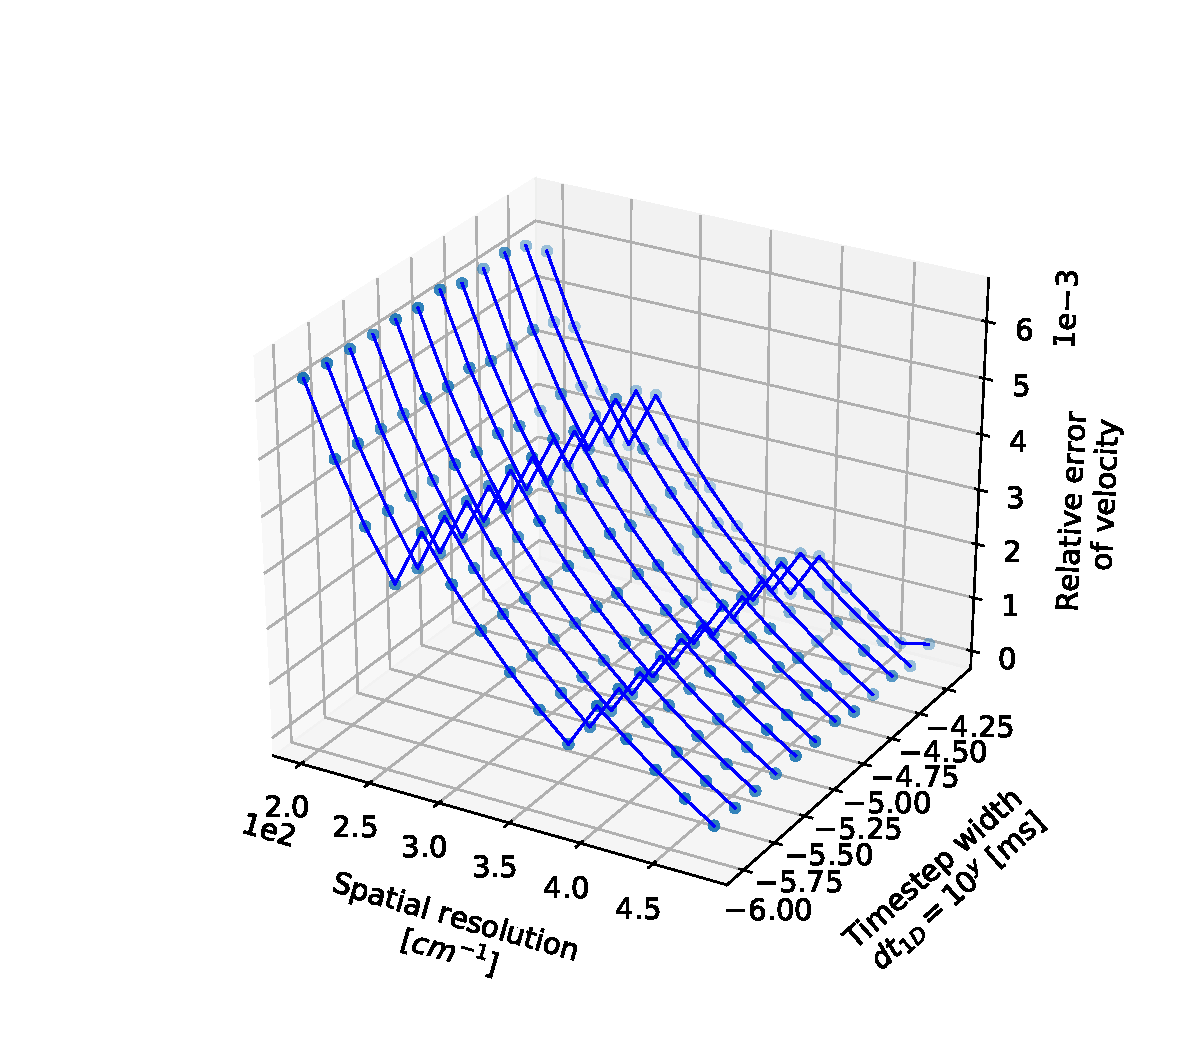
\includegraphics[width=0.8\textwidth]{images/results/studies/hh_cn_error_propagation_velocity_3d.pdf}%
  \caption{Error of the action potential propagation velocity for varying mesh width and timestep width.}% 
   \label{fig:hh_cn_error_propagation_velocity_3d}%
\end{figure}
%-----
\subsection{Linear Solvers for the Multidomain Problem}\label{sec:multidomain_solvers}

% in opendihu 2021 paper
% selected multidomain solvers
\begin{figure}[H]
  \centering%
  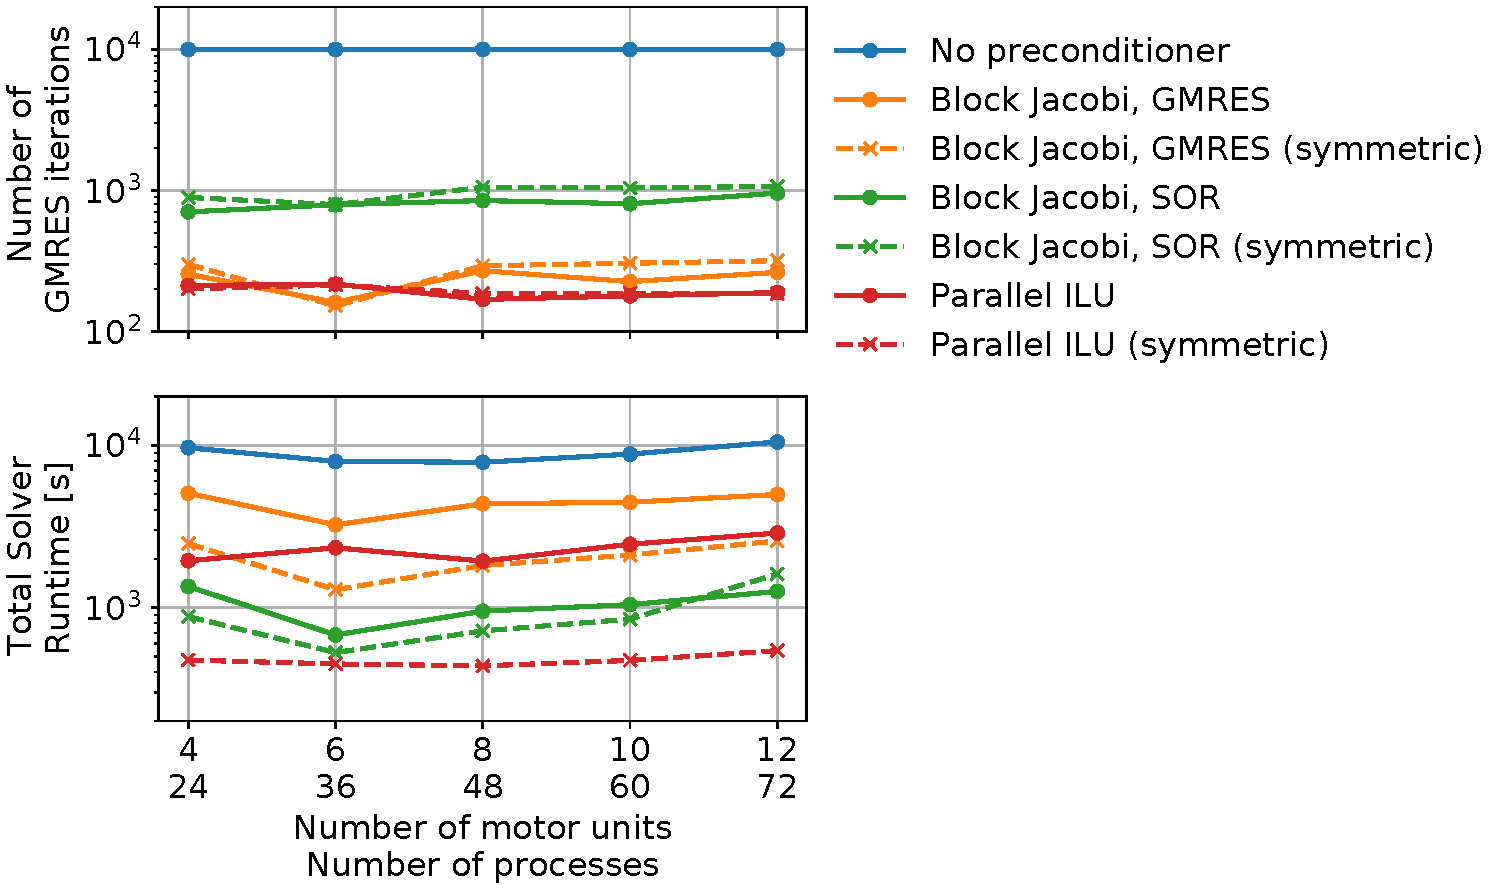
\includegraphics[width=\textwidth]{images/results/studies/multidomain_solvers_selected.pdf}%
  \caption{Multidomain solvers}%
  \label{fig:multidomain_solver}%
\end{figure}

In the next study, we investigate the parallel weak scaling behavior for the multidomain model with fat domain, i.e. \cref{eq:multi-domain1,eq:multi-domain2,eq:subcellular,eq:body} or models (b1),(c) and (d) in \cref{fig:multi-scale-model}. The subcellular model of Shorten et al. \cite{Shorten2007} is used. The goal is to evaluate different preconditioners for the linear solution of the system of equations. The model is discretized by a Strang operator splitting with Heun's method for the subcellular model and an implicit Euler scheme for the multidomain equations. The timestep widths of all schemes are $dt_\text{0D}=dt_\text{multidomain}=dt_\text{splitting}=\SI{5e-4}{\milli\second}$, the end time is \SI{1e-1}{\milli\second}.

We partition the 3D domain of a \num{50024}-node muscle mesh and a \num{37000}-node fat mesh with 24, 36, 48, 60 and 72 processes and simulate 4,6,8,10 and 12 MUs.
As the square-shaped system matrix contains one row of blocks for every MU plus one row of blocks for the fat mesh, the total number of rows scales nonlinearly with the number of MUs. In consequence, the system matrices in the scenarios contain \num{279720}, \num{379768}, \num{479816}, \num{579864} and \num{679912} rows and columns.

% n dofs
% 24: 279720
% 36: 379768
% 48: 479816
% 60: 579864 
% 72: 679912

We solve the linear system of the multidomain equations by a GMRES solver, because the system matrix is non-symmetric.
 The stopping threshold on the residual norm is set to \num{1e-15} and the specified maximum number of iterations is \num{1e4}. 
 \Cref{fig:multidomain_solver} shows the number of GMRES iterations in the upper plot and the total runtimes of the preconditioner and solver in the lower plot.

For every preconditioner, the preconditioning is either performed using the non-symmetric system matrix (solid lines) or using a symmetric matrix that is obtained by taking all diagonal blocks of the system matrix (dashed lines).

The reference measurement is given by using no preconditioner. 
It can be seen that the specified tolerance is not achieved and the maximum number of \num{1e4} iterations is reached.

Two versions of the block Jacobi preconditioner of PETSc are evaluated.
The block Jacobi divides the system matrix into blocks of smaller problems that are each solved individually. 
The first variant uses a GMRES solver, the second variant uses a SOR (successive over relaxation) solver, i.e., a Gauss-Seidel scheme. 
Another solver is ''Euclid`` \cite{euclid} from the HYPRE package, a parallel implementation of incomplete LU factorization using graph partitioning and a two-level ordering strategy.


% scenarioName                                                                 nRanks                                                                                                              
% gmres_bjacobi_dt0.0005_atol1e-15_rtol1e-15_theta1.0_symFalse_lumpFalse_10mus 60      [6, 1, 10]   4444.074833   4472.546500  13.081118   4458.698333     -28.471667    0.0    226.0  0.997 GB  60
% gmres_bjacobi_dt0.0005_atol1e-15_rtol1e-15_theta1.0_symFalse_lumpFalse_12mus 72      [6, 1, 12]   4953.106806   4992.944583  14.215069   4977.854306     -39.837778    0.0    263.0  1.026 GB  72
% gmres_bjacobi_dt0.0005_atol1e-15_rtol1e-15_theta1.0_symFalse_lumpFalse_4mus  24       [4, 1, 6]   5050.243750   5081.276667  11.882062   5068.834583     -31.032917    0.0    255.0  1.389 GB  24
% gmres_bjacobi_dt0.0005_atol1e-15_rtol1e-15_theta1.0_symFalse_lumpFalse_6mus  36       [4, 1, 9]   3234.057500   3248.998333  12.351108   3235.983889     -14.940833    0.0    161.0  0.841 GB  36
% gmres_bjacobi_dt0.0005_atol1e-15_rtol1e-15_theta1.0_symFalse_lumpFalse_8mus  48       [6, 1, 8]   4328.314167   4374.314375  12.322344   4361.300417     -46.000208    0.0    270.0  1.087 GB  48
% gmres_bjacobi_dt0.0005_atol1e-15_rtol1e-15_theta1.0_symTrue_lumpFalse_10mus  60      [6, 1, 10]   2088.741667   2122.034500  13.006847   2108.233667     -33.292833    0.0    305.0  1.074 GB  60
% gmres_bjacobi_dt0.0005_atol1e-15_rtol1e-15_theta1.0_symTrue_lumpFalse_12mus  72      [6, 1, 12]   2549.413056   2589.060139  14.305833   2573.819167     -39.647083    0.0    318.0  1.120 GB  72
% gmres_bjacobi_dt0.0005_atol1e-15_rtol1e-15_theta1.0_symTrue_lumpFalse_4mus   24       [4, 1, 6]   2478.502500   2493.367083  11.744517   2481.051667     -14.864583    0.0    300.0  1.542 GB  24
% gmres_bjacobi_dt0.0005_atol1e-15_rtol1e-15_theta1.0_symTrue_lumpFalse_6mus   36       [4, 1, 9]   1299.019722   1301.245000  12.244350   1288.295833      -2.225278    0.0    152.0  0.827 GB  36
% gmres_bjacobi_dt0.0005_atol1e-15_rtol1e-15_theta1.0_symTrue_lumpFalse_8mus   48       [6, 1, 8]   1801.928542   1830.392917  12.377065   1817.272500     -28.464375    0.0    293.0  1.069 GB  48
% gmres_euclid_dt0.0005_atol1e-15_rtol1e-15_theta1.0_symFalse_lumpFalse_10mus  60      [6, 1, 10]   2489.941833   2471.670167  13.204272   2457.642167      18.271667    0.0    179.0  0.510 GB  60
% gmres_euclid_dt0.0005_atol1e-15_rtol1e-15_theta1.0_symFalse_lumpFalse_12mus  72      [6, 1, 12]   2914.482639   2895.433472  14.660654   2879.770000      19.049167    0.0    189.0  0.551 GB  72
% gmres_euclid_dt0.0005_atol1e-15_rtol1e-15_theta1.0_symFalse_lumpFalse_4mus   24       [4, 1, 6]   1974.359167   1954.868333  11.758821   1942.513750      19.490833    0.0    212.0  0.473 GB  24
% gmres_euclid_dt0.0005_atol1e-15_rtol1e-15_theta1.0_symFalse_lumpFalse_6mus   36       [4, 1, 9]   2366.323333   2349.646111  12.330914   2336.598333      16.677222    0.0    217.0  0.437 GB  36
% gmres_euclid_dt0.0005_atol1e-15_rtol1e-15_theta1.0_symFalse_lumpFalse_8mus   48       [6, 1, 8]   1963.516458   1945.901875  12.508950   1932.620625      17.614583    0.0    169.0  0.471 GB  48
% gmres_euclid_dt0.0005_atol1e-15_rtol1e-15_theta1.0_symTrue_lumpFalse_10mus   60      [6, 1, 10]    506.561333    486.702183  13.177800    472.658200      19.859150    0.0    187.0  0.470 GB  60
% gmres_euclid_dt0.0005_atol1e-15_rtol1e-15_theta1.0_symTrue_lumpFalse_12mus   72      [6, 1, 12]    577.824583    558.374014  14.584994    542.841681      19.450569    0.0    185.0  0.518 GB  72
% gmres_euclid_dt0.0005_atol1e-15_rtol1e-15_theta1.0_symTrue_lumpFalse_4mus    24       [4, 1, 6]    509.154167    487.713333  11.844267    475.261125      21.440833    0.0    201.0  0.448 GB  24
% gmres_euclid_dt0.0005_atol1e-15_rtol1e-15_theta1.0_symTrue_lumpFalse_6mus    36       [4, 1, 9]    480.553056    462.281917  12.279769    449.267556      18.271139    0.0    214.0  0.409 GB  36
% gmres_euclid_dt0.0005_atol1e-15_rtol1e-15_theta1.0_symTrue_lumpFalse_8mus    48       [6, 1, 8]    469.558750    450.701521  12.482108    437.435708      18.857229    0.0    186.0  0.433 GB  48
% gmres_none_dt0.0005_atol1e-15_rtol1e-15_theta1.0_symFalse_lumpFalse_10mus    60      [6, 1, 10]   8697.286500   8841.893667  14.195788   8826.917167    -144.607167    0.0  10000.0  2.184 GB  60
% gmres_none_dt0.0005_atol1e-15_rtol1e-15_theta1.0_symFalse_lumpFalse_12mus    72      [6, 1, 12]  10342.686111  10501.216667  15.572006  10484.729167    -158.530556    0.0  10000.0  2.536 GB  72
% gmres_none_dt0.0005_atol1e-15_rtol1e-15_theta1.0_symFalse_lumpFalse_4mus     24       [4, 1, 6]   9229.770417   9675.692083  14.665854   9660.403333    -445.921667    0.0  10000.0  2.006 GB  24
% gmres_none_dt0.0005_atol1e-15_rtol1e-15_theta1.0_symFalse_lumpFalse_6mus     36       [4, 1, 9]   7886.560833   7975.463611  13.603492   7961.178056     -88.902778    0.0  10000.0  1.982 GB  36
% gmres_none_dt0.0005_atol1e-15_rtol1e-15_theta1.0_symFalse_lumpFalse_8mus     48       [6, 1, 8]   7728.828542   7876.260625  13.214875   7862.334583    -147.432083    0.0  10000.0  2.145 GB  48
% gmres_sor_dt0.0005_atol1e-15_rtol1e-15_theta1.0_symFalse_lumpFalse_10mus     60      [6, 1, 10]   1064.128667   1056.613667  13.017858   1042.770333       7.515000    0.0    805.0  0.514 GB  60
% gmres_sor_dt0.0005_atol1e-15_rtol1e-15_theta1.0_symFalse_lumpFalse_12mus     72      [6, 1, 12]   1282.427083   1274.231389  14.543176   1258.699861       8.195694    0.0    959.0  0.572 GB  72
% gmres_sor_dt0.0005_atol1e-15_rtol1e-15_theta1.0_symFalse_lumpFalse_4mus      24       [4, 1, 6]   1314.639167   1366.876250  15.078050   1351.132917     -52.237083    0.0    705.0  0.470 GB  24
% gmres_sor_dt0.0005_atol1e-15_rtol1e-15_theta1.0_symFalse_lumpFalse_6mus      36       [4, 1, 9]    703.937778    691.388333  12.411444    678.247556      12.549444    0.0    793.0  0.433 GB  36
% gmres_sor_dt0.0005_atol1e-15_rtol1e-15_theta1.0_symFalse_lumpFalse_8mus      48       [6, 1, 8]    972.381875    963.809000  12.346906    950.696875       8.572875    0.0    849.0  0.511 GB  48
% gmres_sor_dt0.0005_atol1e-15_rtol1e-15_theta1.0_symTrue_lumpFalse_10mus      60      [6, 1, 10]    869.906333    862.904083  13.149073    848.941350       7.002250    0.0   1042.0  0.553 GB  60
% gmres_sor_dt0.0005_atol1e-15_rtol1e-15_theta1.0_symTrue_lumpFalse_12mus      72      [6, 1, 12]   1606.299028   1628.942917  17.998925   1609.921528     -22.643889    0.0   1070.0  0.575 GB  72
% gmres_sor_dt0.0005_atol1e-15_rtol1e-15_theta1.0_symTrue_lumpFalse_4mus       24       [4, 1, 6]    917.225833    896.343042  14.958108    880.731083      20.882792    0.0    893.0  0.495 GB  24
% gmres_sor_dt0.0005_atol1e-15_rtol1e-15_theta1.0_symTrue_lumpFalse_6mus       36       [4, 1, 9]    552.407222    540.981389  12.264922    527.989472      11.425833    0.0    794.0  0.452 GB  36
% gmres_sor_dt0.0005_atol1e-15_rtol1e-15_theta1.0_symTrue_lumpFalse_8mus       48       [6, 1, 8]    739.617708    732.262771  12.567985    718.927312       7.354937    0.0   1055.0  0.526 GB  48


% ==============
%\iffalse
% --------------
%-----
\section{Parallel in Time master thesis}
maybe
%-----
%-----
\section{Output file sizes}
no
%-----
%\section{Mesh convergence, stochastic with different MU assignments}
%-----
\section{dx-dt dependencies} 
no
%-----
\section{Load balancing bachelor thesis}
no
%-----
\section{Application of opendihu within the field of robotics} 
no

\chapter{Conclusion and Future Work}\label{sec:conclusion_and_future_work}

\section{Future Work}\label{sec:future_work}
 
% more timestepping methods: CVODE (https://computing.llnl.gov/projects/sundials/cvode), imex
% different parallelisation where not all ranks have to be involved (for multidomain) -> this feature already exists for the fibers with multipleInstances
% more numeric tests on exp function? no


% ------------
%\fi
% f===========

